\documentclass[a4paper,12pt]{article}
\usepackage[top=2.5cm,bottom=2.5cm,left=2.5cm,right=2.5cm]{geometry}
%% \usepackage[brazil,brazilian]{babel}
\usepackage{amsmath, nccmath}
\usepackage{amsfonts}
\usepackage{amssymb}
\usepackage{multirow}
\usepackage{natbib}
\usepackage[colorlinks,citecolor=blue,urlcolor=blue]{hyperref}
\usepackage[utf8]{inputenc}
\usepackage{graphicx}  
\usepackage{float}
\usepackage{pdflscape} % horizontal page
\usepackage{tabularx}
\usepackage[english,vlined,ruled]{algorithm2e}
\usepackage{booktabs}
\usepackage{tikz}
\usetikzlibrary{positioning,shapes,arrows}
\usepackage{adjustbox}
\usepackage{tikz}
\usetikzlibrary{backgrounds}
\usetikzlibrary{arrows}
\usetikzlibrary{shapes,shapes.geometric,shapes.misc}

% this style is applied by default to any tikzpicture included via \tikzfig
\tikzstyle{tikzfig}=[baseline=-0.25em,scale=0.5]

% these are dummy properties used by TikZiT, but ignored by LaTex
\pgfkeys{/tikz/tikzit fill/.initial=0}
\pgfkeys{/tikz/tikzit draw/.initial=0}
\pgfkeys{/tikz/tikzit shape/.initial=0}
\pgfkeys{/tikz/tikzit category/.initial=0}

% standard layers used in .tikz files
\pgfdeclarelayer{edgelayer}
\pgfdeclarelayer{nodelayer}
\pgfsetlayers{background,edgelayer,nodelayer,main}

% style for blank nodes
\tikzstyle{none}=[inner sep=0mm]

% include a .tikz file
\newcommand{\tikzfig}[1]{%
{\tikzstyle{every picture}=[tikzfig]
\IfFileExists{#1.tikz}
  {\input{#1.tikz}}
  {%
    \IfFileExists{./figures/#1.tikz}
      {\input{./figures/#1.tikz}}
      {\tikz[baseline=-0.5em]{\node[draw=red,font=\color{red},fill=red!10!white] {\textit{#1}};}}%
  }}%
}

% the same as \tikzfig, but in a {center} environment
\newcommand{\ctikzfig}[1]{%
\begin{center}\rm
  \tikzfig{#1}
\end{center}}

% fix strange self-loops, which are PGF/TikZ default
\tikzstyle{every loop}=[]

\usepackage{setspace}
\onehalfspacing

\title{
  
  A multinomial generalized linear mixed model for clustered competing
  risks data

}
\author{
  Henrique Aparecido Laureano\thanks{
    Laborat\'{o}rio de Estat\'{i}stica e Geoinforma\c{c}\~{a}o,
    Departamento de Estat\'{i}stica,
    Universidade Federal do Paran\'{a}, Curitiba, Brasil.
    E-mail: laureano@ufpr.br
  }~
  Wagner Hugo Bonat$^\ast$}
 
\begin{document}
\maketitle

\begin{abstract}

  Clustered competing risks data are a complex failure time data
  scheme. Its main characteristics are the cluster structure, which
  implies a latent within-cluster dependence between its elements, and
  its multiple variables competing to be the one responsible for the
  occurrence of an event, the failure. To handle this kind of data, we
  propose a full likelihood approach, based on a generalized linear
  mixed model instead a usual complex frailty model. We model the
  competing causes in the probability scale, in terms of the cumulative
  incidence function (CIF). A multinomial distribution is assumed for
  the competing causes and censorship, conditioned on the latent
  effects. The latent effects are accommodated via a multivariate
  Gaussian distribution. The CIF is specified as the product of an
  instantaneous risk level function with a failure time trajectory level
  function. The estimation procedure is performed through the R package
  TMB (Template Model Builder), an \texttt{C++} based framework with
  efficient Laplace approximation and automatic differentiation
  routines. A large simulation study is performed, based on different
  latent structure formulations. The model presents to be of difficult
  estimation, with our results converging to a latent structure where
  the risk and failure time trajectory levels are correlated.

\end{abstract}
\vfill
\noindent\textbf{Keywords}: 
Clustered competing risks data;
Within-cluster dependence;
Multinomial generalized linear mixed model (GLMM);
TMB: Template Model Builder;
Laplace approximation;
Automatic differentiation (AD).
\vspace{0.2cm}
\newpage

\section{Introduction}

Failure time data is the branch of Statistics responsible to handle
random variables describing the time until the occurrence of an event, a
failure \citep{kalb&prentice,hougaard00}. The time until a failure is
called survival experience, and is the modeling object. To accommodate
the number of possible causes for a failure there is the competing risks
data scheme, described in Figure \ref{fig:crp} and the focus of this
work. More specifically, its clustered version i.e., with groups of
elements sharing some non-observed latent dependence structure.

\begin{figure}[H]
 \centering
 \scalebox{0.85}{
  \begin{tikzpicture}
   \begin{pgfonlayer}{nodelayer}
    \node [style=circle,draw=black,fill=white] (7) at (-7.5, 5.5) {1};
    \node [style=circle,draw=black,fill=white] (9) at (-7.5, 4.5) {2};
    \node [style=none] (11) at (-7.5, 3.5) {$\vdots$};
    \node [style=circle,draw=black,fill=white] (12) at (-7.5, 2.5) {$m$};
    \node [style=circle,draw=black,fill=white] (14) at (-12.25, 4) {0};
    \node [style=none] (29) at (-11.75, 4.25) {};
    \node [style=none] (30) at (-8, 5.5) {};
    \node [style=none] (31) at (-8, 4.5) {};
    \node [style=none] (32) at (-8, 2.5) {};
    \node [style=none] (36) at (-11.75, 4) {};
    \node [style=none] (37) at (-11.75, 3.75) {};
   \end{pgfonlayer}
   \begin{pgfonlayer}{edgelayer}
	\draw [style=1side] (37.center) to (32.center);
	\draw [style=1side] (36.center) to (31.center);
	\draw [style=1side] (29.center) to (30.center);
   \end{pgfonlayer}
  \end{tikzpicture}
 }
 \caption{Illustration of competing risks process.}
 \label{fig:crp}
\end{figure}

The survival experiences is usually modeled in the hazard (failure rate)
scale, and with the latent within-cluster dependence accommodation we
have a frailty model \citep{frailty78,frailty79,liang95,petersen98}. The
use of frailty models implies complicated likelihood functions and
inference routines done via elaborated and slow EM algorithms
\citep{nielsen92,klein92} or inefficient MCMC schemes
\citep{hougaard00}. With multiple survival experiences, the general idea
is the same but with even more elaborated likelihoods
\citep{prentice78,therneau00} or using instead mixture model approaches
\citep{larson85,kuk92}.

When in the hazard scale, the interpretations are in terms of hazard
rates. A less usual scale but with a more appealing interpretation, is
to model the survival experiences in the probability scale. For
competing risks data, the work on the probability scale is done by means
of the cumulative incidence function (CIF) \citep{andersen12}, with the
main modeling approach being the subdistribution \citep{fine&gray}.

For clustered competing risks data there are some available options but
with a lack of predominance. The options vary in terms likelihood
specification, with its majority being designed for bivariate CIFs,
where increasing the CIF's dimension is a limitation. Some of the
existing options are (i) nonparametric approaches
\citep{cheng07,cheng09}; (ii) linear transformation models
\citep{fine99,gerds12}; (iii) semiparametric approaches based on
composite likelihoods \citep{shih,SCHEIKE}, estimating equations
\citep{crossoddsratioSCHEIKE,cheng&fine}, copulas
\citep{semiparametricSCHEIKE}, and mixtures \citep{naskar05,shi13}.

Besides the interpretation, by modeling the CIF possible to specify
complex within-cluster dependence structures. We follow \cite{SCHEIKE}
and work with a CIF specification based on its decomposition in
instantaneous risk and failure time trajectory, with both being
cluster-specifics and possible correlated. As a modeling framework, we
use a generalized linear mixed model (GLMM) specification.

The class of generalized linear models (GLMs) \citep{GLM72} is probably
the most popular statistical modelling framework. Despite its
flexibility, the GLMs are not suitable for dependent data. For the
analysis of such data, \cite{laird82} proposed the random effects
regression models for longitudinal/repeated-measures data
analysis. \cite{breslow93} presented the GLMMs for the analysis of
non-Gaussian outcomes. In this framework, we can accommodate all
competing causes of failure and censorship with a multinomial
probability distribution, easily extend to any number of competing
causes. The within-cluster dependence is accommodated via a multivariate
normal distribution and the cause-specific CIFs via the model's link
function. The estimation and inference are done via an efficient
implementation and state-of-art computational libraries provided through
TMB. The latent effects are handled out by means of an efficient Laplace
approximation and automatic differentiation.

The main goal of this study is to propose a GLMM approach to handle
clustered competing risks data with a flexible within-cluster dependence
structure. The model specification and the inferential routine are much
simpler than the usually used approaches, increasing the practical
relevance of our framework. The estimation and inference is made through
the efficient computational resources of the R \citep{R21} package
\texttt{TMB} \citep{TMb}.

The main contributions of this article are: (i) introducing the modeling
of cause/cluster-specific CIFs of clustered competing risks data into an
efficient implementation of the GLMMs framework; (ii) performing a
extensive simulation study to check the properties of the maximum
likelihood estimator to learn the cause-specific CIF forms and the
feasibility of the within-cluster dependence structure.; (iii) providing
R code and \texttt{C++} implementation for the used GLMMs.

The work is organized as follows. Section \ref{model} presents the CIF
specification and the multinomial GLMM. Section \ref{inference} presents
the estimation and inferential routines. Section \ref{simulation}
presents the performed simulation studies to check the model
viability. Finally, the main contributions of the article are discussed
in Section \ref{discussion}.

\section{Model}
\label{model}

\begin{figure}[H]
 \centering 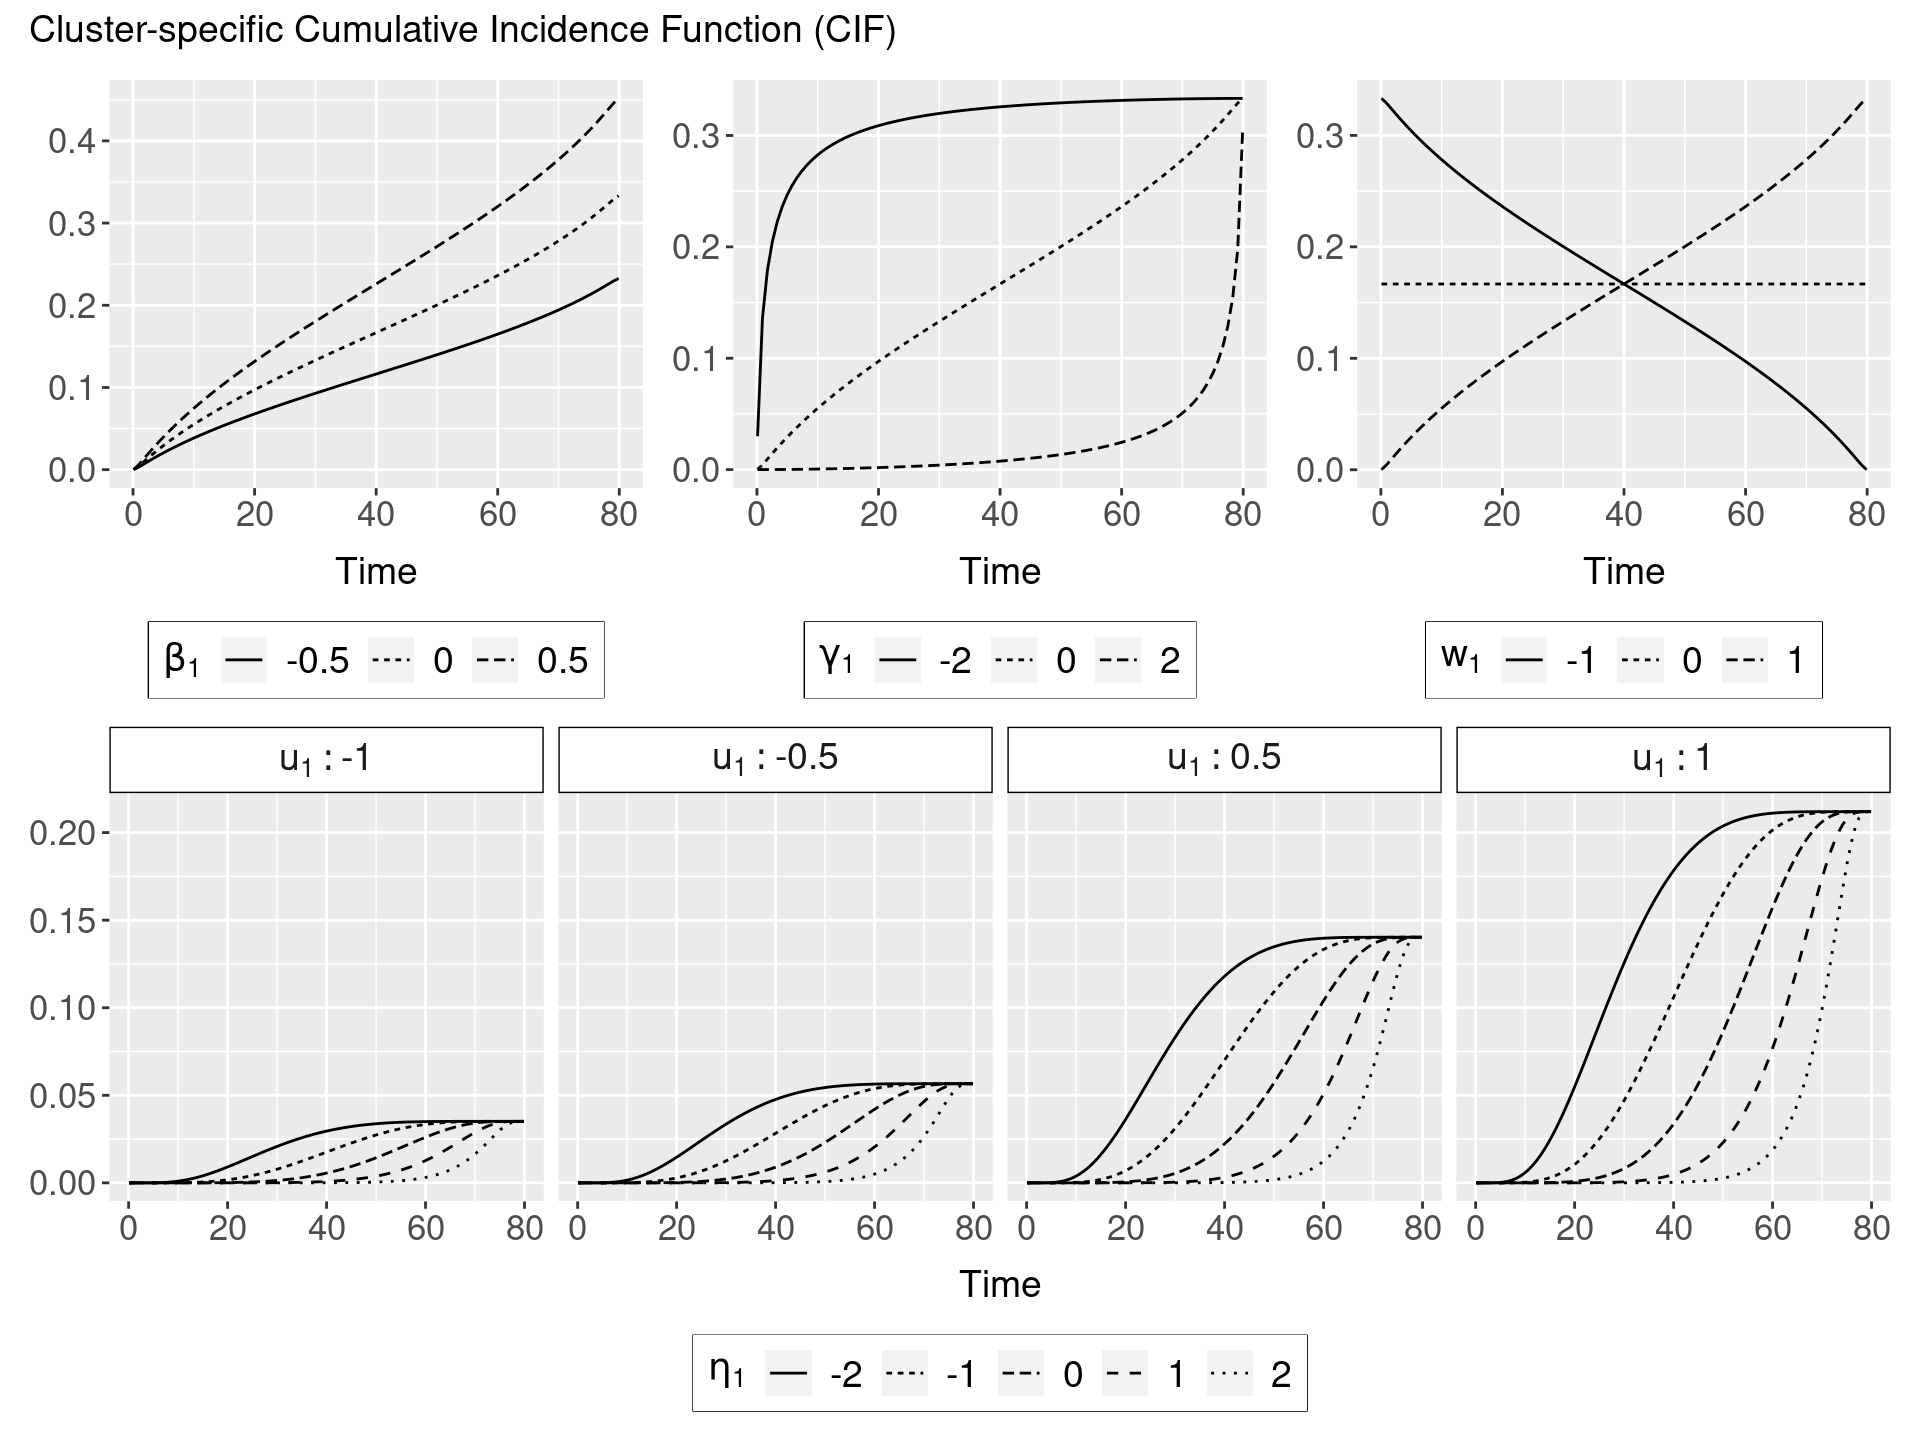
\includegraphics[width=\linewidth]{pics/cifstudy-1.png}
 \vspace{-0.75cm}
 \caption{Curve behaviors for different parameter settings, showing then
   the corresponding parameter effects in a cluster-specific cumulative
   incidence function (CIF).}
 \label{fig:cifcoefs}
\end{figure}

\section{Estimation and inference}
\label{inference}

\section{Simulation studies}
\label{simulation}

\section{Discussion}
\label{discussion}

\section*{Supplementary material}

\bibliographystyle{dcu}
\bibliography{references}

\end{document}
